\appendix

% \section{Appendix / supplemental material}
\section{Appendix}

\subsection{Limitations.}
One limitation of our approach lies in the reduced "receptive field" compared to methods that perform dense computation over the entire local search region. By focusing on a smaller set of motion-guided tokens, the model may miss targets that move abruptly or unpredictably outside the attended area. This issue becomes more pronounced if the underlying model lacks sufficient accuracy, or if the input frame rate is too low—leading to poor motion continuity and large inter-frame displacements. In such scenarios, the tracker may fail to recover the target, resulting in decreased performance. Future work may explore adaptive mechanisms to dynamically adjust the search area or incorporate long-term cues to address these challenges.

\subsection{Per-Atrribute Analysis.}
The radar chart in \figref{radar} shows that 30\% tokens with a motion window (blue) achieve performance close to 100\% tokens (red) across most attributes, especially in fast motion and occlusion scenarios. In contrast, 30\% tokens without a motion window (cyan) exhibit notable drops in attributes like out-of-view and background clutter. The decline in background clutter performance may stem from the model's insufficient discriminative capability, leading to the predicted bounding box drifting toward similar objects. When this inaccurate prediction is used to generate the motion window, it restricts the search area, further limiting the model's ability to recover the target in cluttered backgrounds. This shows the need for stronger discriminative features to complement sparsification strategies.

 \begin{figure}[h]
% \vskip -0.4in
\begin{center}
\centerline{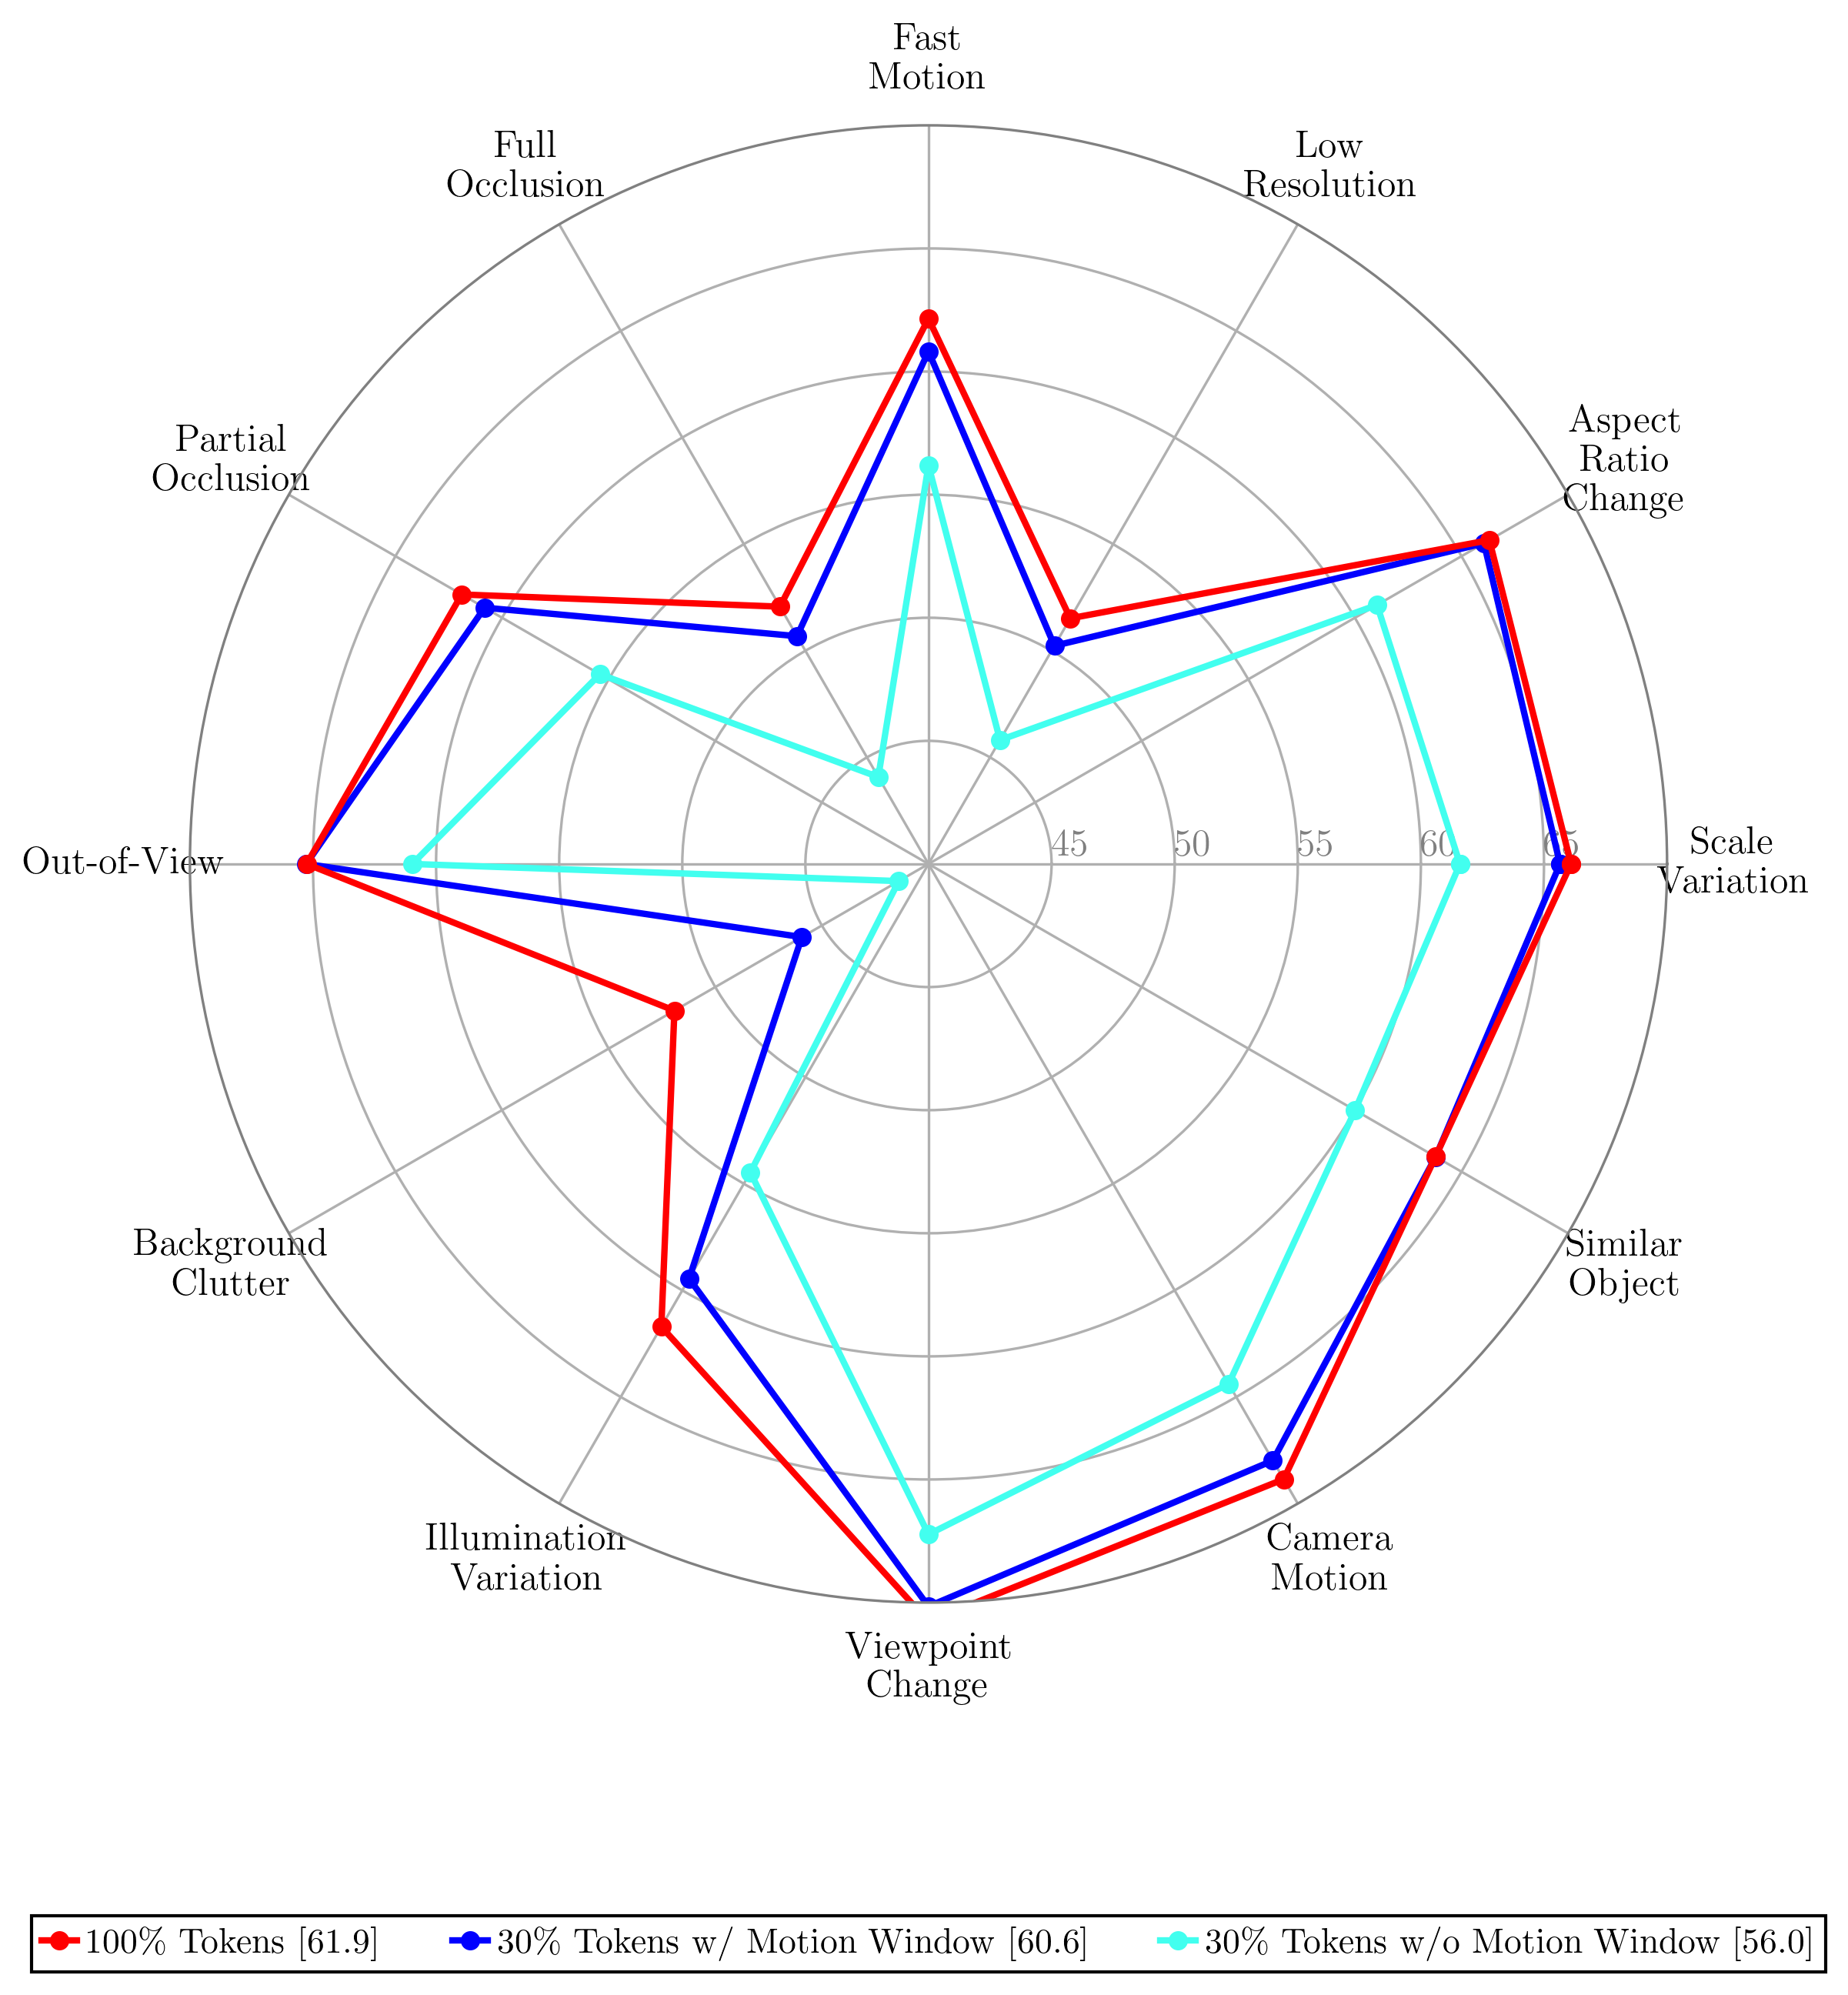
\includegraphics[width=0.7\columnwidth]{imgs/radar_plot.png}}
\caption{Per-attribute performance comparison using a radar chart. Results are shown for three setups: 100\% tokens, 30\% tokens with motion window, and 30\% tokens without motion window. The motion window significantly improves performance in challenging scenarios like fast motion, occlusion, and out-of-view cases.}
\label{radar}
\end{center}
% \vskip -0.4in
\end{figure}

\subsection{Analysis of Motion Window.}
\tabref{tab:windowing} presents an ablation study of various windowing strategies used in the proposed framework. We compare two window types (Gaussian and Cosine), evaluate the effect of incorporating cross-attention importance scores, and analyze whether dynamic window resizing (based on the width and height of the previous frame’s bounding box) improves performance. Results show that combining importance scores with a Gaussian window achieves the best overall performance. The fiexd windowing approach yields sub-optimal perfrmance compared to dynamic window sizes. The last two rows highlight that using only motion windows for sparsification performs better than using only cross-attention scores, but their combination consistently outperforms either individually. This confirms that both the spatial prior and cross-attention scores are crucial for effective token selection.
This conclusion is further supported by \figref{abl_vs}, where the orange solid line (Gaussian with motion windows) achieves superior AUC across different token retention rates compared to the dashed orange line (without motion windows). The motion window effectively enhances the selection of relevant tokens, particularly at lower retention rates (e.g., 30\% and 20\%), where its use maintains accuracy while achieving higher FPS. This demonstrates the importance of combi`ning spatial priors from motion windows with cross-attention scores to optimize tracking performance and efficiency.

\begin{table}[ht]
    \centering
    \caption{Comparison of different windowing strategies on GOT-10k \texttt{val}. We evaluate the impact of window type (Gaussian or Cosine), the use of importance scores, and whether the window dynamically adapts to the previous frame’s bounding box size and aspect ratio.}
    \resizebox{0.9\linewidth}{!}{
        \begin{tabular}{c|c|c|ccc}
            \toprule
            {Window} & \multirow{2}{*}{\shortstack{Importance                                   \\Score}} & \multirow{2}{*}{Dynamic} & \multirow{2}{*}{AUC} & \multirow{2}{*}{P} & \multirow{2}{*}{P$_{Norm}$}\\
            {Type}   &                                        &            &      &             \\
            \midrule[0.5pt]
            Gaussian & \checkmark                             & \checkmark & 79.9 & 71.7 & 91.5 \\
            Gaussian & \checkmark                             & -          & 79.5 & 70.5 & 90.2 \\
            Cosine   & \checkmark                             & \checkmark & 79.8 & 71.1 & 91.2 \\
            Cosine   & \checkmark                             & -          & 79.1 & 70.2 & 89.9 \\
            -        & \checkmark                             & -          & 76.9 & 68.2 & 86.5       \\
            Gaussian & -                                      & \checkmark & 78.2 & 69.1 & 88.1      \\
            % \hline
            % Gaussian       & \checkmark                & 25\%                 & 68.2              & 75.4   \\
            % Cosine         & \checkmark                & 25\%                 & 67.9              & 76.8   \\
            % -           & \checkmark                & 25\%                 & 65.8              & 80.5   \\
            % Gaussian       & -                & 25\%                 & 62.3              & 82.9   \\ 
            \bottomrule
        \end{tabular}}
    \label{tab:windowing}
\end{table}

\subsection{Scaling to Larger Models and Resolutions.}
Experiments shown in ~\tabref{tab:scaling} examine the scalability of our motion-aware sparsification by applying it to a slightly larger ViT-Base model(LoRAT~\cite{lorat}) and increasing the input resolution from 256×256 to 384×384. This experiment demonstrates the generalizability of our approach to larger models and higher-resolution inputs.

\begin{table}[ht]
    \centering
    \caption{Results of scaling to a ViT-Base model and increasing input resolution. Accuracy (Acc) and FPS are reported.}
    \resizebox{0.7\linewidth}{!}{
        \begin{tabular}{c|c|c|cc|c}
            \toprule
            Model & Input                    & \%Tokens Retained & LaSOT & GOT-10k & FPS \\
                  &                          &                   & AUC   & AO      & (GPU)   \\
            \midrule[0.5pt]
            \multirow{6}*{\shortstack{ViT-base}}
                  & \multirow{2}*{\(224^2\)} & 100\%             & 71.3  & 71.9    & 116 \\
                  &                          & 30\%              & 69.8  & 70.2    & 215 \\
            \cline{2-6}
                  & \multirow{4}*{\(378^2\)} & 100\%             & 72.1  & 73.3    & 51  \\
                  &                          & 30\%              & 70.4  & 71.5    & 104 \\
                  &                          & 20\%              & 68.9  & 70.6    & 119 \\
                  &                          & 10\%              & 67.2  & 68.4    & 126 \\

            \bottomrule
        \end{tabular}}
    \label{tab:scaling}
\end{table}


\subsection{Running Latency on More Platforms.}
Our primary focus is on real-world deployment scenarios, particularly on edge devices, where power consumption and thermal constraints are critical factors. High-power GPUs, while useful for benchmarking, are often impractical for real-world applications in embedded and mobile settings.  \tabref{tab:fps_more} reports the inference speed (in FPS) and accuracy (LaSOT AUC) of several tracking methods across four representative hardware platforms. The benchmark shows that MaST still get a better trade-off between accuracy and speed even on powerful devices.

\begin{table}[ht]
    \centering
    \caption{Comparison of tracking speed (FPS) for different methods on various hardware platforms, including NVIDIA 2080Ti GPU, Intel i7-13700 CPU, intel N100, and Raspberry Pi 5 (RPi-5). LaSOT AUC is reported as a measure of accuracy.}
    \resizebox{0.7\linewidth}{!}{
        \begin{tabular}{c|c|cccc}
            \toprule
            Method& LaSOT AUC& 2080Ti & i7-13700 & N100 & RPi-5 \\
            \midrule[0.5pt]
            MaST-tiny                       & 63.3  & 453    & 184      & 48.3 & 22.6  \\
MaST-nano                       & 58.6  & 511    & 205      & 64.5 & 30.1  \\
HiT-T                           & 59.1  & 355    & 176      & 53.3 & 27.3  \\
HiT-S                           & 60.5  & 309    & 144      & 43.5 & 21.5  \\
LightTrack                      & 53.8  & 444    & 136      & 60.2 & 13.4  \\
AVTrack                         & 64.1  & 274    & 78       & 17.3 & 7.7       \\
            % \hline
            % Gaussian       & \checkmark                & 25\%                 & 68.2              & 75.4   \\
            % Cosine         & \checkmark                & 25\%                 & 67.9              & 76.8   \\
            % -           & \checkmark                & 25\%                 & 65.8              & 80.5   \\
            % Gaussian       & -                & 25\%                 & 62.3              & 82.9   \\ 
            \bottomrule
        \end{tabular}}
    \label{tab:fps_more}
\end{table}


\subsection{More Visualizations.}
1. Rapid Motion Scenario: The visualization of \figref{fig:vis1} demonstrates that MaST (30\% tokens with motion window) can robustly track rapidly moving objects, closely matching the performance of the full-token model (100\% tokens). In contrast, a naive sparsification strategy without the motion-aware component fails completely. This clearly illustrates the crucial role of our motion-aware sparsification in handling rapid motion cases.

2. Failure Cases under Extremely Challenging Conditions: We acknowledge there exist extreme conditions, e.g., low-quality UAV footage with significant appearance ambiguity in \figref{fig:vis2}, that surpass the capability of even the full-token model. Such difficulties are fundamentally challenging for existing state-of-the-art trackers, not limited to MaST. Therefore, performance degradation under these conditions stems from inherent limitations common to the tracking domain rather than from sparsification or motion-aware strategies.

 \begin{figure}[h]
% \vskip -0.4in
\begin{center}
\centerline{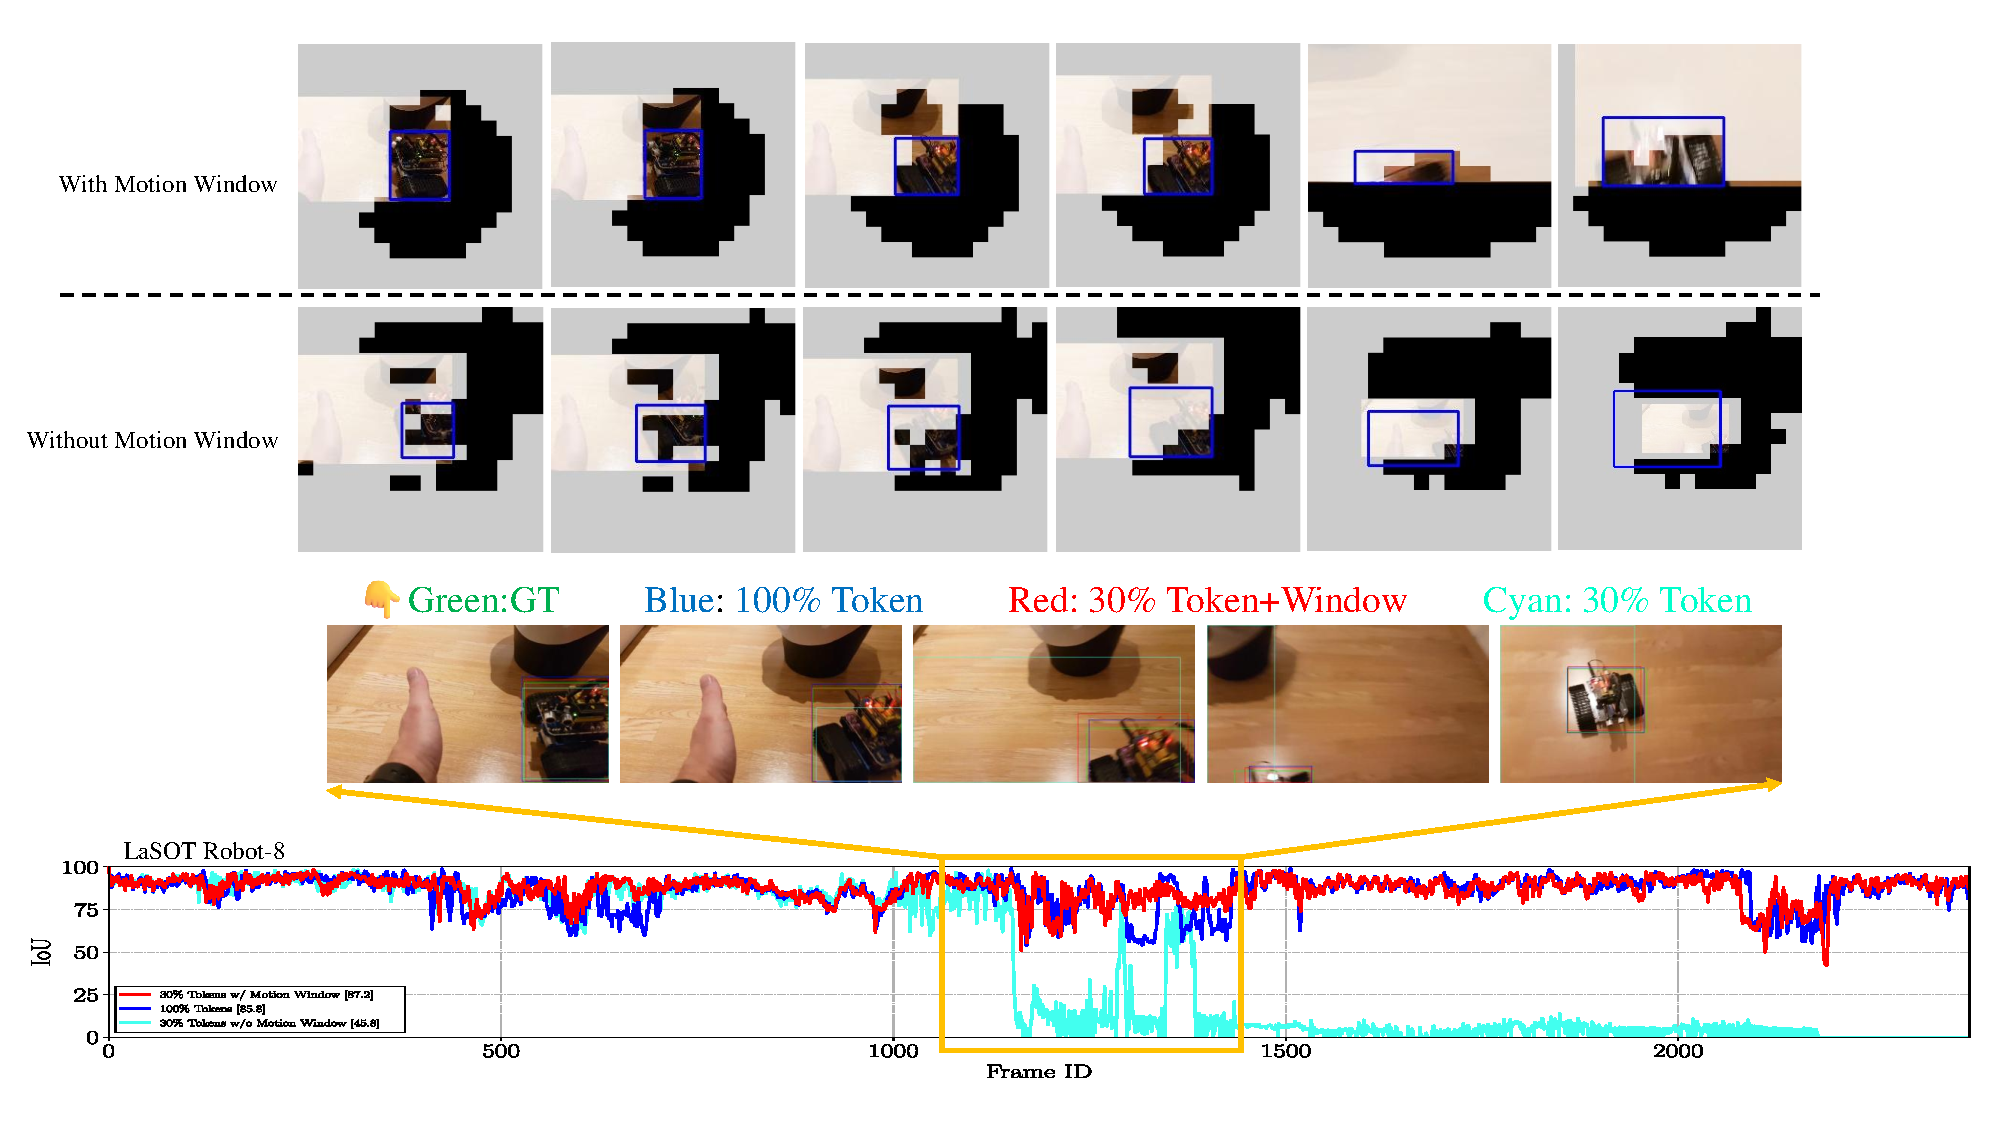
\includegraphics[width=0.98\columnwidth]{imgs/video_vis1.pdf}}
\caption{Tracking a robot when it engage fast movement, leading to partially out-of-view.  Sparsification without motion-aware fixing would quickly discard the features of the target, making the tracker focus on other objects in the view.}
\label{fig:vis1}
\end{center}
\end{figure}

 \begin{figure}[h]
% \vskip -0.4in
\begin{center}
\centerline{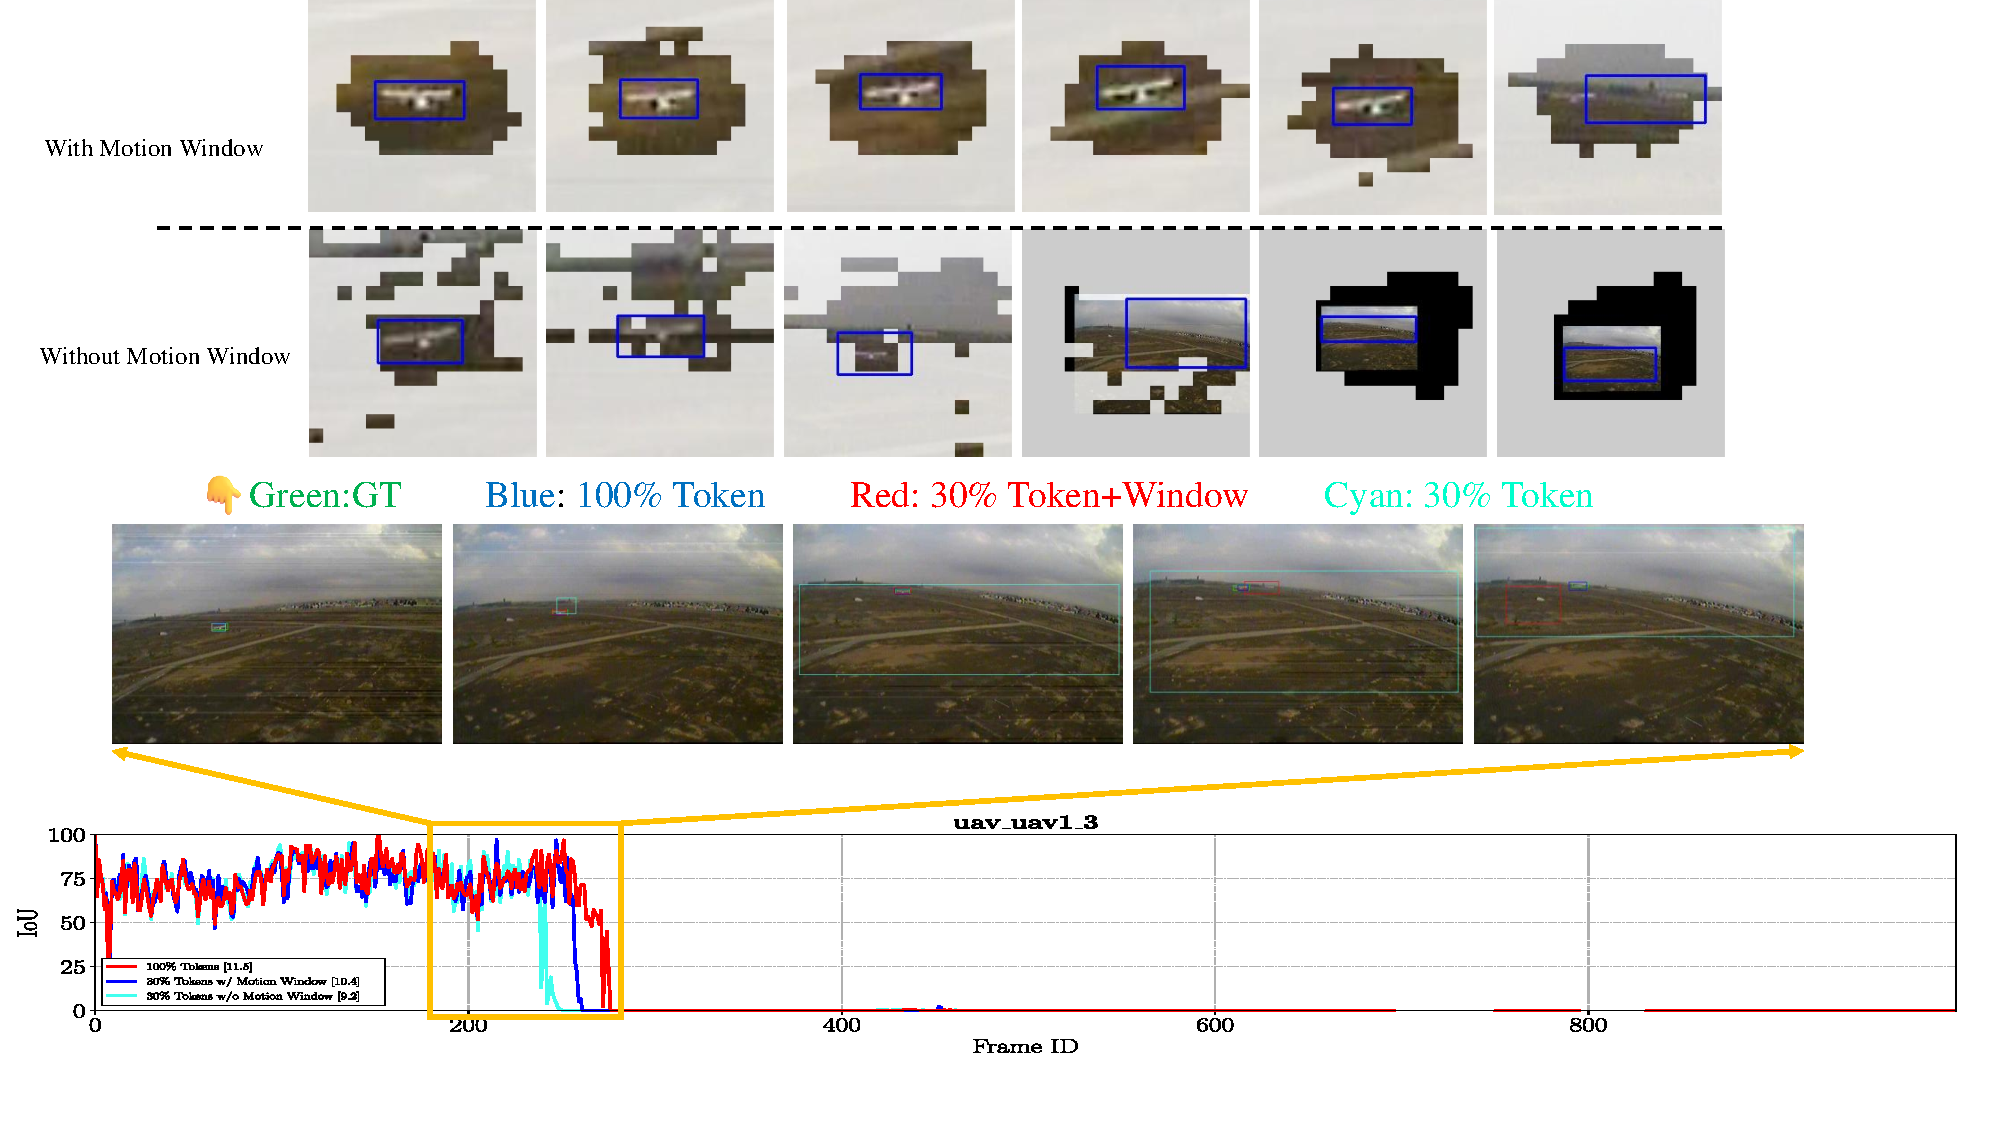
\includegraphics[width=0.98\columnwidth]{imgs/video_vis2.pdf}}
\caption{Handling small objects like UAVs under extremely bad situation.  With or without sparsification or motion-aware sparsification, the tracker is difficult to keep tracking the target.}
\label{fig:vis2}
\end{center}
\end{figure}

\clearpage